\section{Results}

Initially, a baseline model (ground truth only) was trained with an
early stopping mechanism, which stopped the training when the
validation loss stopped decreasing for 10 epochs, reaching only 20
epochs of significant training. The results are shown in Figure
\ref{fig:baseline_segment_20_epochs}.

Then, using the scalar model described in Section
\ref{sec:scalar_model}, training
was performed for 20 epochs and Bayesian hyperparameter optimization
on learning rate,
decoder dropout rate, for the regularizers described in
Section \ref{sec:regularizers}. The results are shown in Figure
\ref{fig:crowd_seg_scalar_model_overfitting}.

\begin{figure}[H]
  \centering
  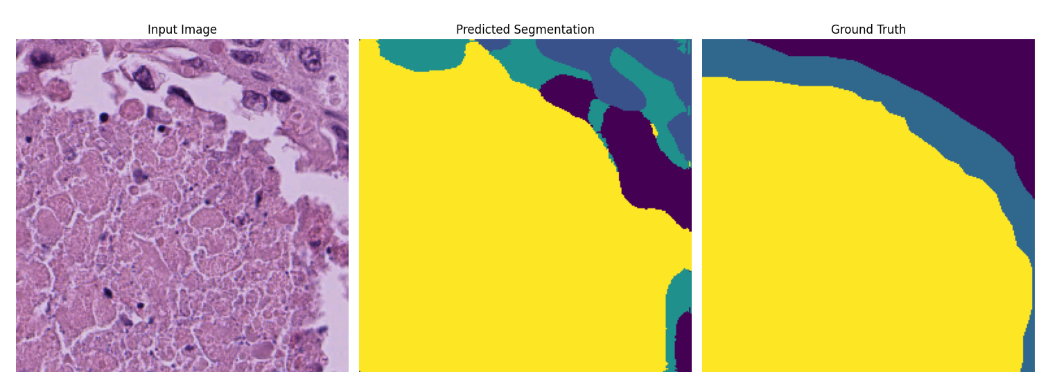
\includegraphics[
  width=0.8\textwidth]{Cap5/Figures/baseline_segment_20_epochs.png}
  \caption{Segmentation results for baseline model on the \gls{TNBC}
    (Crowd-Seg) dataset after 20 epochs of training. Even though the
    segmentation algorithm seems to show progress on its way to capture
    the underlying target structures ot be segmented, since the ground
    truth annotation is not expressive enough, the Dice coefficient
    remains below 0.55, which is not considered a good performance.
    The baseline model remained with overfitting even after combining
    techniques of: Bayesian hyperparameter optimization, data
    augmentation, learning rate scheduling, dataset shuffling, and
  early stopping.}
  \label{fig:baseline_segment_20_epochs}
\end{figure}

\begin{figure}[H]
  \centering
  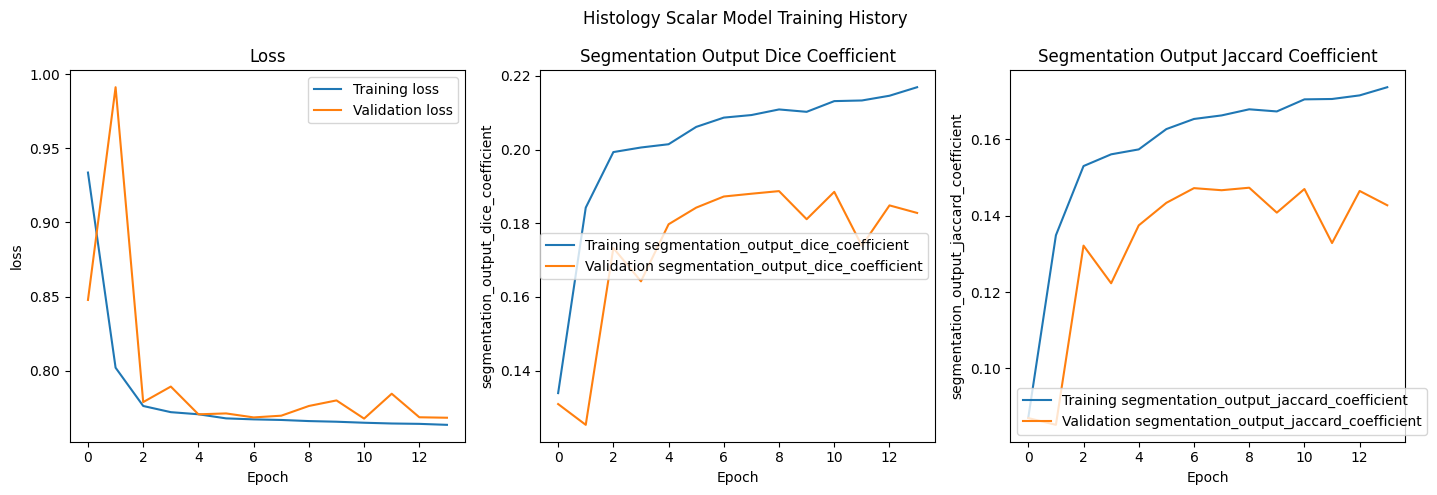
\includegraphics[
  width=0.8\textwidth]{Cap5/Figures/crowd_seg_scalar_model_overfitting.png}
  \caption{Segmentation results for scalar model on the \gls{TNBC}
    (Crowd-Seg) dataset after 20 epochs of training. Again, training
    metrics show a constant grow, but not validation metrics, which
  shows a combined issue of overfitting and unreliable ground truth.}
  \label{fig:crowd_seg_scalar_model_overfitting}
\end{figure}

\subsection{Oxford-IIIT Pet Dataset}

The experimental results on the Oxford-IIIT Pet Dataset demonstrate
interesting insights into the performance of different approaches.
While STAPLE achieves the highest Dice and Jaccard scores (0.8718 and
0.7917 respectively) for the dataset with no missing labels (label
rate of 1.0), our proposed TGCE$_{SS}$ approaches show superior
performance for label rates below 1.0 (Table \ref{tab:oxford_pet_results}).
The pixel-wise variant, while slightly lower in performance metrics,
provides more detailed spatial reliability information. It is of note
that the key strength of TGCE$_{SS}$ lies in its ability to
simultaneously learn both segmentation and reliability estimation,
providing valuable insights into annotator behavior and confidence
levels that STAPLE and MV cannot offer.
\begin{table}[h]
  \centering
  \begin{tabular}{lcccccc}
    \hline
    \textbf{Method} & \multicolumn{2}{c}{\textbf{Label Rate 1.0}} &
    \multicolumn{2}{c}{\textbf{Label Rate 0.7}} &
    \multicolumn{2}{c}{\textbf{Label Rate 0.3}} \\
    & Dice & Jaccard & Dice & Jaccard & Dice & Jaccard \\
    \hline
    TGCE scalar   & 0.8658±0.009 & 0.7838±0.012 &
    \textbf{0.8566±0.017} & \textbf{0.7724±0.024} &
    \textbf{0.8529±0.004} & \textbf{0.7677±0.007} \\
    TGCE feature  & 0.8629±0.044 & 0.7806±0.047 & 0.8528±0.026 &
    0.7664±0.027 & 0.8458±0.026 & 0.7569±0.027 \\
    TGCE pixel    & 0.8603±0.018 & 0.7767±0.025 & 0.8545±0.013 & %
    % unchanged pixel lr=.5
    0.7695±0.017 & 0.8283±0.001 & 0.7359±0.002 \\
    MV            & 0.8132±0     & 0.7222±0     & 0.7572±0     &
    0.6554±0     & 0.5566±0     & 0.4687±0 \\
    STAPLE        & \textbf{0.8718±0} & \textbf{0.7917±0} & 0.8439±0
    & 0.7609±0     & 0.5734±0     & 0.5158±0 \\
    \hline
  \end{tabular}
  \caption{Performance metrics (Dice and Jaccard) at different
  labeling rates. Best values per category are bolded.}
  \label{tab:oxford_pet_results}
\end{table}

The reliability estimation capabilities of our model are particularly
noteworthy, as demonstrated in Figures
\ref{fig:oxford_example_output} and
\ref{fig:oxford_example_output_pixel}. The model successfully
captures the varying reliability levels of different annotators, with
higher reliability assigned to annotators with lower noise levels (10
dB) and lower reliability to those with higher noise levels (-20 dB).
This ability to quantify and visualize annotator reliability is a
significant advantage over traditional approaches like STAPLE and MV,
which focus solely on segmentation accuracy without providing
insights into annotator behavior.

\begin{figure}[H]
  \centering
  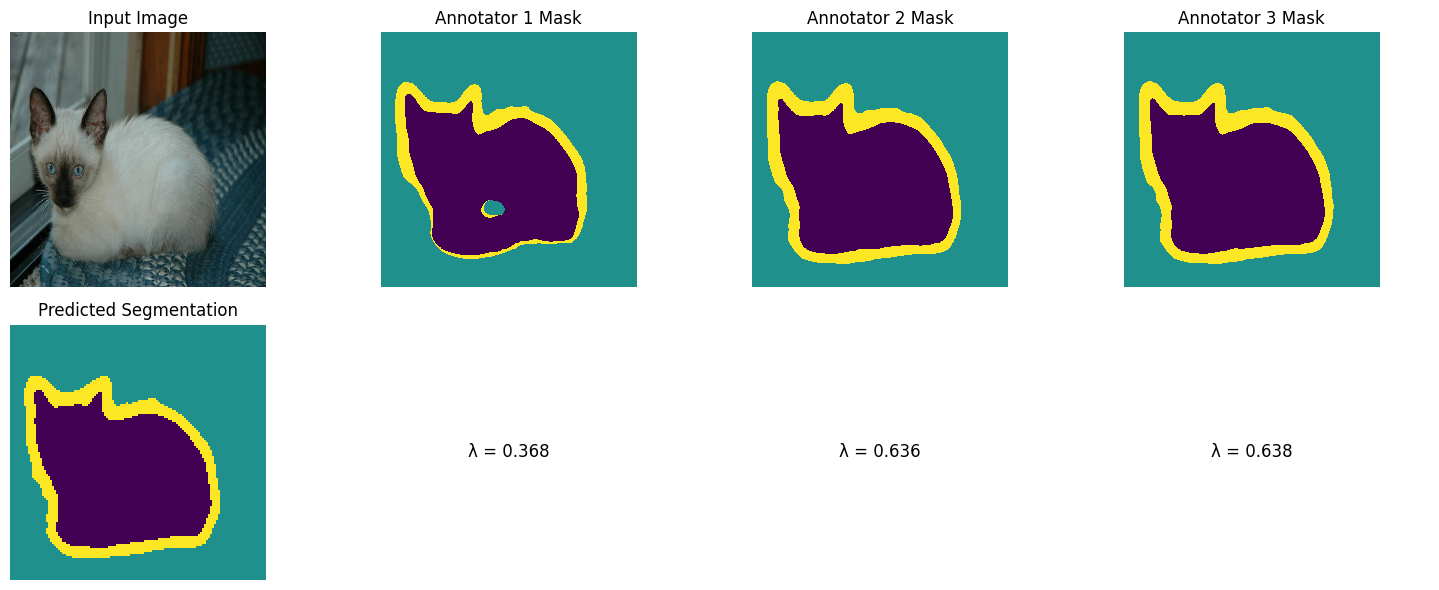
\includegraphics[width=0.8\textwidth]{Cap5/Figures/oxford_example_output_scalar.png}
  \caption{Example evaluation of the proposed model in its last
    trained epoch. An accurate segmentation output is delivered as well
    as scalar reliability estimations from the labelers masks.
    Disturbance signal-to-noise ratios are: $[-20, 0, 10]$ dB from
    left to right.
    Best found hyperparameters: learning rate = 0.0011, $q = 0.4$,
    noise tolerance = 0.2, $\alpha_{reg} = 0.26$,
  $\alpha_{entropy} = 0.03$, $\alpha_{sum} = 0.27$.}
  \label{fig:oxford_example_output}
\end{figure}

\begin{figure}[H]
  \centering
  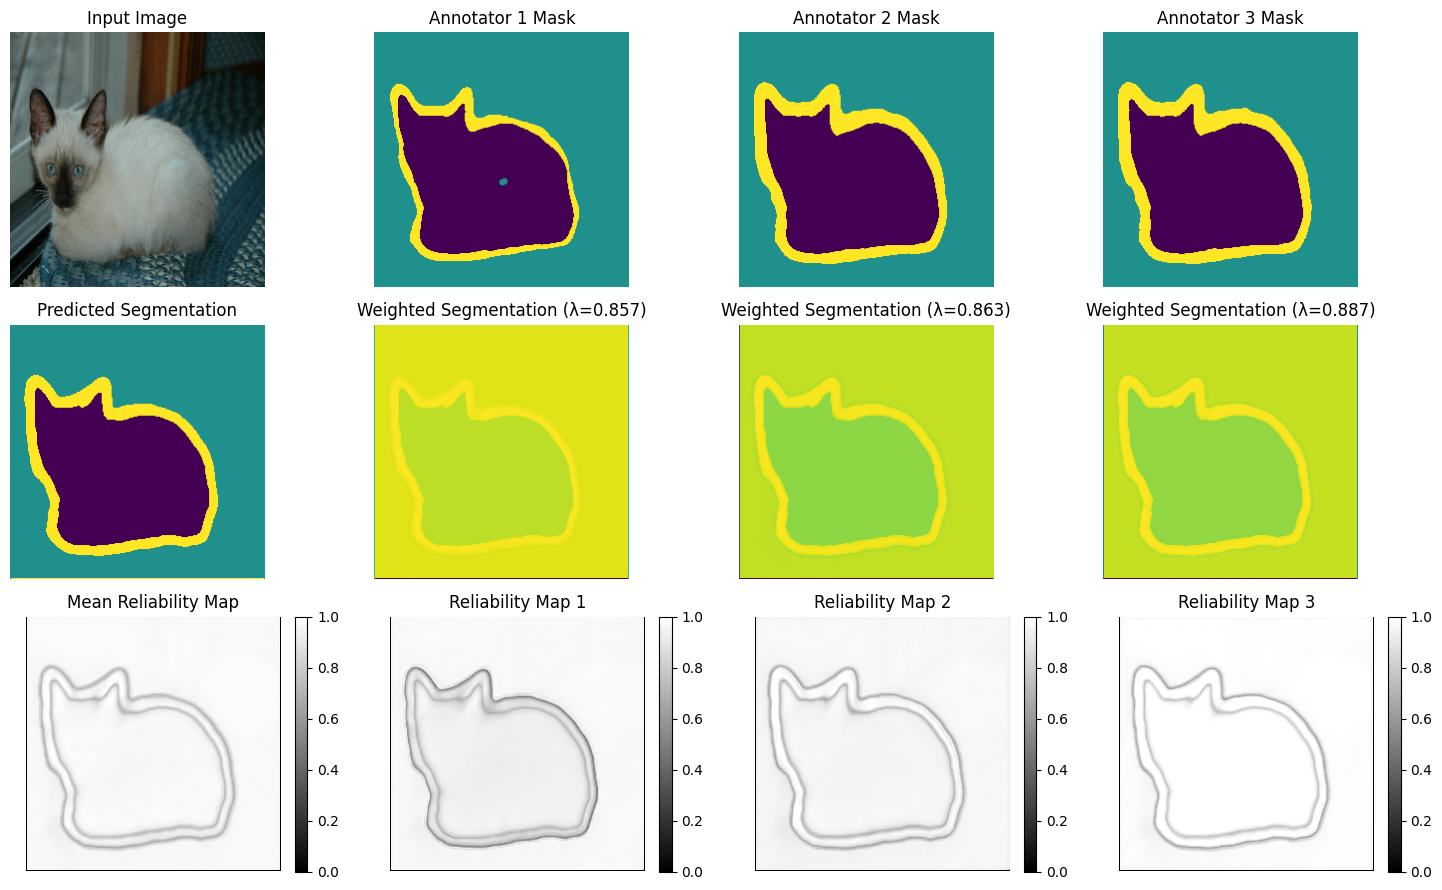
\includegraphics[width=0.8\textwidth]{Cap5/Figures/oxford_example_output_pixel.png}
  \caption{Example evaluation of the proposed model in some given
    epoch (5/50) of training, which demonstrates a quick convergence
    of the model for correctly estimating the reliability of the labelers
    masks. An accurate segmentation output is delivered as well
    as pixel-wise reliability estimations from the labelers masks.
    Disturbance signal-to-noise ratios are: $[-20, 0, 10]$ dB from left
    to right. Best found hyperparameters: learning rate = 0.0027,
    $q = 0.9$, noise tolerance = 0.2, $\alpha_{reg} = 0.38$,
  $\alpha_{entropy} = 0.02$, $\alpha_{sum} = 0.42$.}
  \label{fig:oxford_example_output_pixel}
\end{figure}

\subsection{TNBC Dataset}

As mentioned in Section \ref{sec:tnbc_dataset},
\cite{AmgadEtAl2019} presented
a \gls{TNBC} dataset, which is
crowdsourced and available as HistomicsTK metadata. Later,
\cite{Lopez2023} sampled 151 \glspl{WSI}, from which 161 \glspl{ROI}
were extracted and labeled by 20 medical students. The dataset was
sampled as patches of size 512x512, resulting in 10173 training
patches, 1264 validation patches and 399 testing patches. The
segmentation masks for the patches are composed of the classes:
Tumor, Stroma, Inflammation, Necrosis, and Others \footnote{In
  practice, some of this masks also contain an additional class
labeled as `ignore'.}. This subset of the \gls{TNBC} is named Crowd-Seg
\cite{Lopez2023}.

Raw PNG files for the images patches and masks were provided by the
authors, in practice, in order to optimize the use of these data, a
custom tensorflow dataset was built for facilitating batch memory,
caching and prefetching. The custom dataset implementation handles
the loading and preprocessing of both images and masks, including
normalization of images to the [0,1] range and one-hot encoding of
the segmentation masks. It also manages the multi-annotator structure
by creating a labeler mask that indicates which annotators provided
labels for each sample. The dataset supports data augmentation
through random transformations (flips, rotations, brightness/contrast
adjustments) and includes visualization utilities for debugging and
analysis purposes. This custom dataset implementation is publicly
available \footnote{\url{https://github.com/blotero/seg_tgce}}
\footnote{\url{https://seg-tgce.readthedocs.io/en/latest/}} within
the PyPI package included in the overall solution of this work.
(see Section \ref{sec:academic_discussion}).

\subsubsection{Notes on the Crowd-Seg Dataset}
The multiple labelers version of the \gls{TNBC} dataset (Crowd-Seg)
contains a couple of peculiarities that are worth mentioning.
First, the label rate (inverse percentage of labels that are missing)
is not uniform across the labelers and, in general, quite low, ranging
from 1 to 12\% as seen in Figure \ref{fig:tnbc_label_rates}.

\begin{figure}[H]
  \centering
  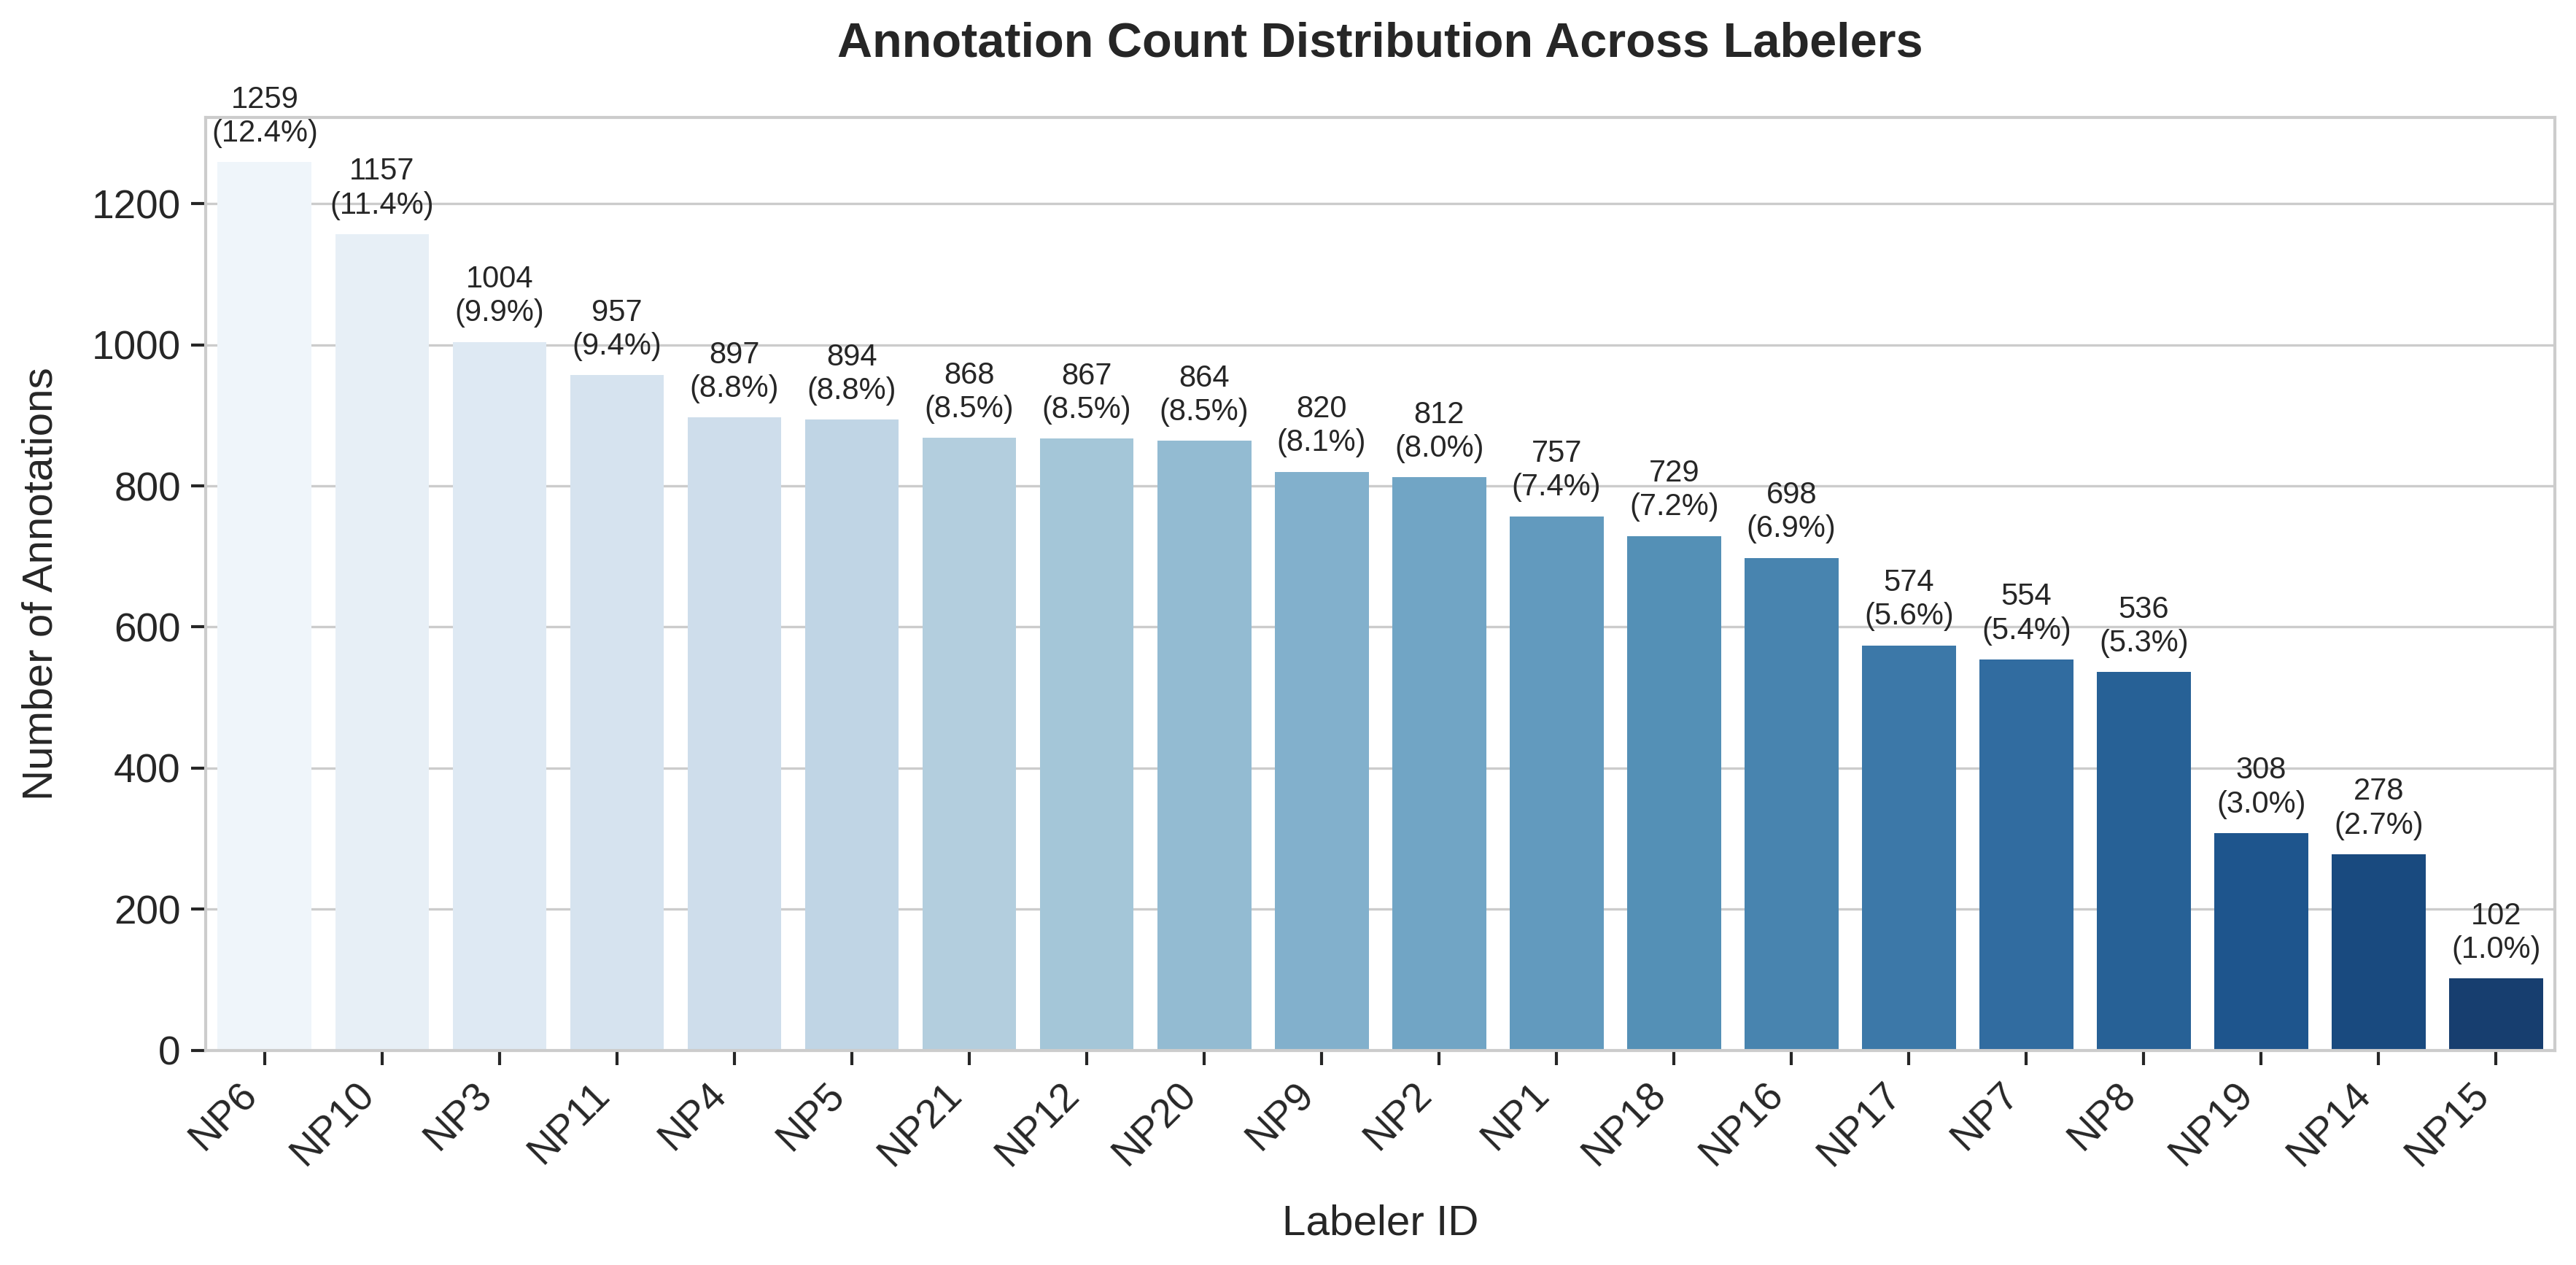
\includegraphics[width=0.9\textwidth]{Cap5/Figures/crowd_seg_annotation_distribution.png}
  \caption{Label rate distribution across the labelers for the \gls{TNBC}
  (Crowd-Seg) dataset.}
  \label{fig:tnbc_label_rates}
\end{figure}

On the other hand, the classes distribution across all patches are
not equal, being `Tumor' (class 2) the most frequent class. Despite
the classes not being equally distributed, the distribution of the
classes across the labelers is fairly uniform, as shown in Figure
\ref{fig:tnbc_labelers_classes_distribution}.

\begin{figure}[H]
  \centering
  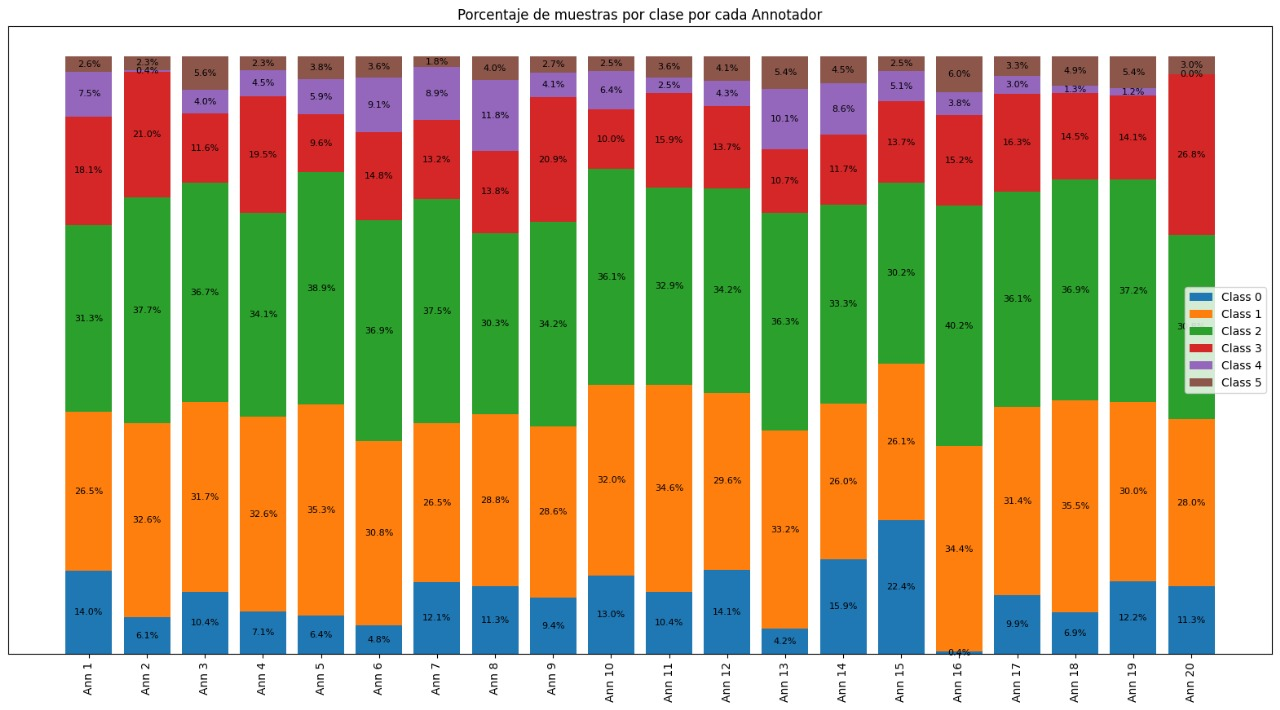
\includegraphics[trim=0pt 0pt 0pt 20pt, clip,
  width=0.8\textwidth]{Cap5/Figures/labelers_classes_distribution_histologies.jpeg}
  \caption{Classes distribution across the labelers for the \gls{TNBC}
    (Crowd-Seg) dataset.
    Most common classes are `Tumor' (class 2),`Other' (class 1) and
  `Stroma' (class 3).}
  \label{fig:tnbc_labelers_classes_distribution}
\end{figure}

It was also found that the dice score of the labelers masks against
the ground truth differed across the labelers and the classes, as
shown in Figure \ref{fig:crowd_seg_annotated_vs_dice}. The target
class (Tumor) ranged dice scores across the labelers from 0.5 to 0.9,
other classes can get as low as 0.4 for in average for some
labelers, meaning
very high levels of disagreement.

\begin{figure}[H]
  \centering
  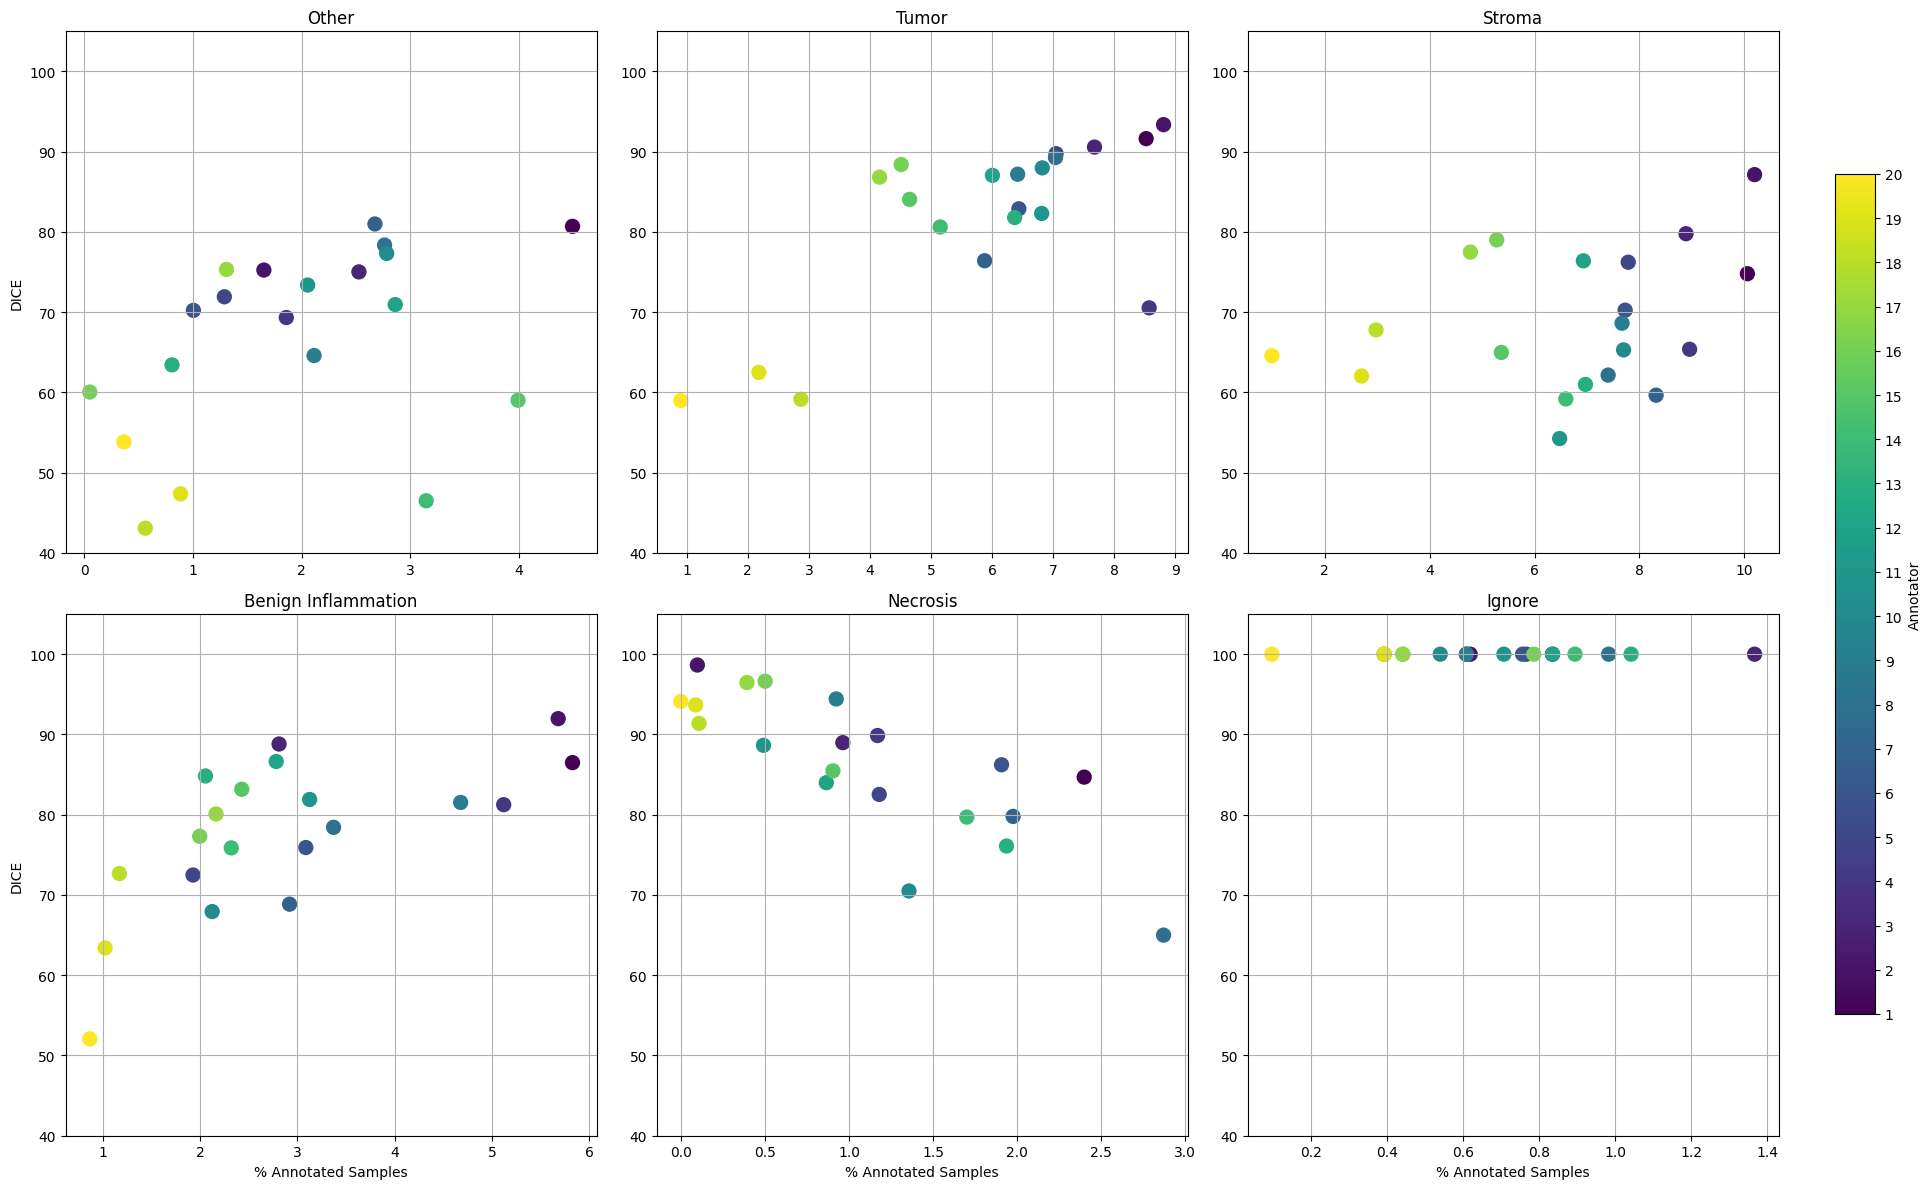
\includegraphics[width=0.8\textwidth]{Cap5/Figures/crowd_seg_annotated_vs_dice.png}
  \caption{Dice score of the labelers masks against the ground truth
  for the \gls{TNBC} (Crowd-Seg) dataset.}
  \label{fig:crowd_seg_annotated_vs_dice}
\end{figure}

Finally, it was found that the expert labels, which would thereby be
considered as ground truth for metrics evaluation, were not always
correct, as shown in Figure \ref{fig:ground_truth_odd_geometries}.
These morphological inconsistencies make an objetive metric for
evaluating the performance of the proposed model difficult to define,
since the ground truth is not always correct or expressive enough.

\begin{figure}[H]
  \centering
  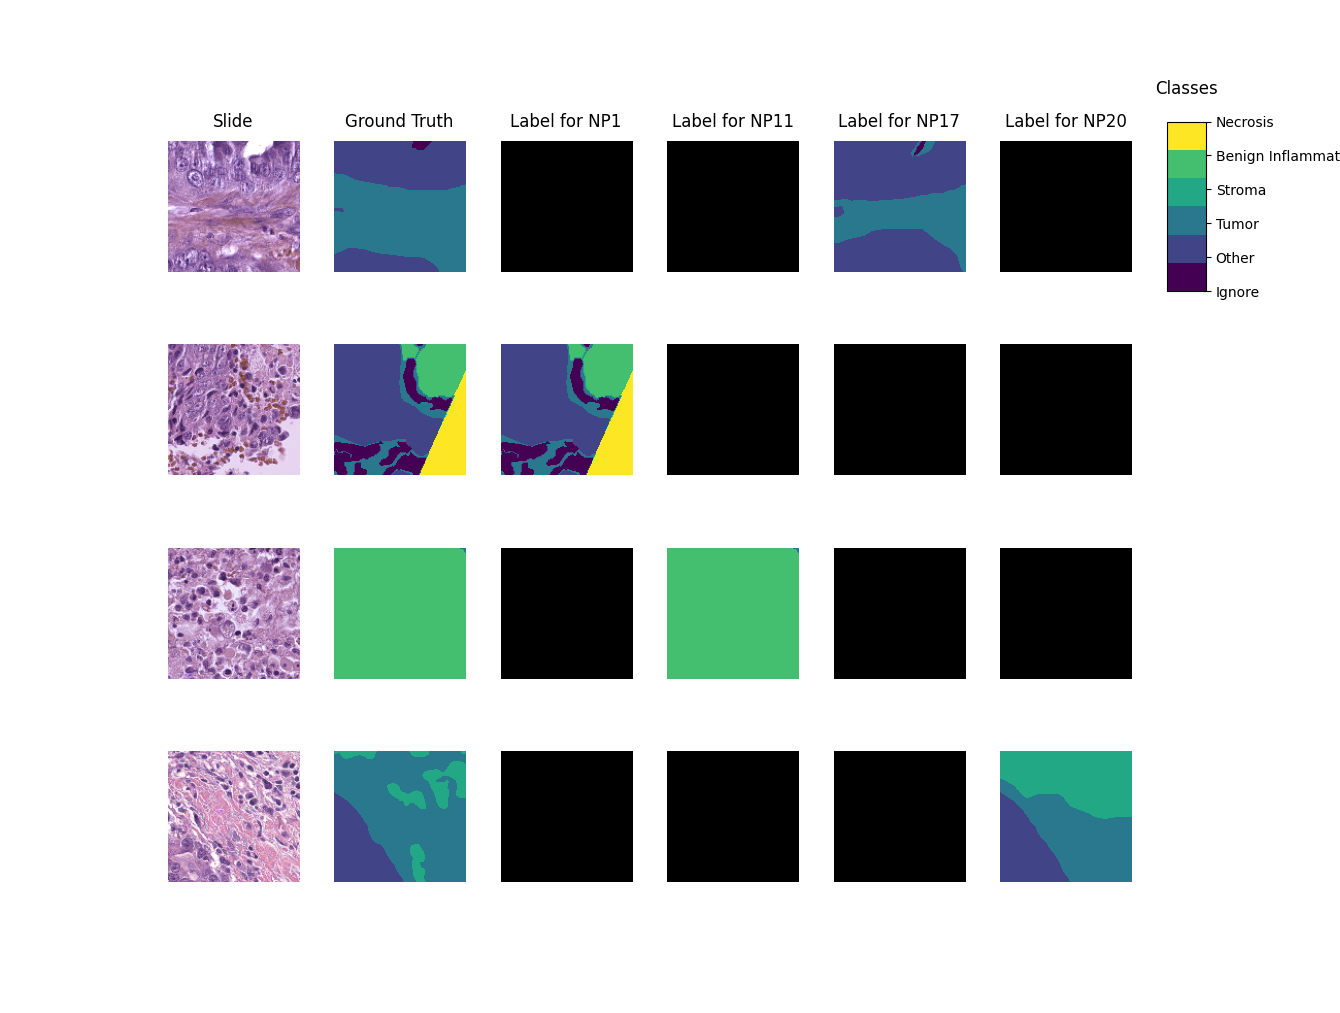
\includegraphics[width=0.8\textwidth]{Cap5/Figures/ground_truth_odd_geometries_2.png}
  \caption{Example of ground truth with odd geometries (second patch
    from top to bottom), which are not always correct or compatible
  with the underlying structures of the patch itself.}
  \label{fig:ground_truth_odd_geometries}
\end{figure}

\begin{figure}[H]
  \centering
  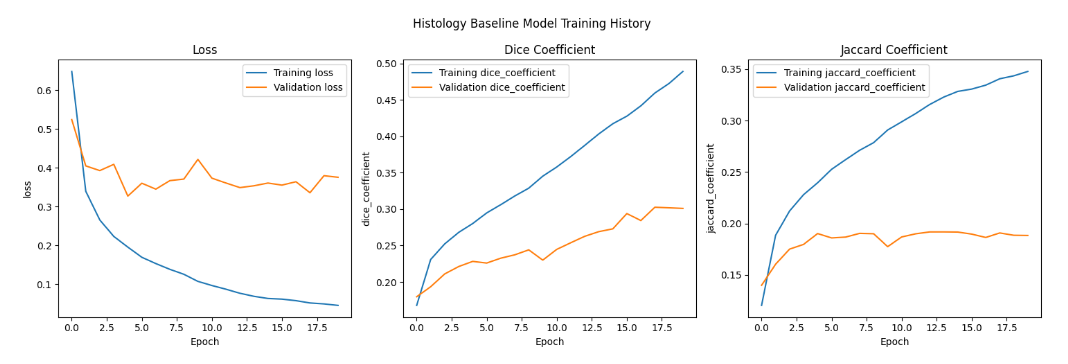
\includegraphics[
  width=0.8\textwidth]{Cap5/Figures/crowd_seg_baseline_training_curves.png}
  \caption{Training curves for the baseline model on the \gls{TNBC}
  (Crowd-Seg) dataset.}
  \label{fig:tnbc_baseline_training_curves}
\end{figure}
